\section{Bounded-oscillation languages}
\label{sec:osc}
Bounded-oscillation languages were introduced by Ganty and Valput \cite{BoundOsc}. Just like one-counter and linear languages, it is defined by restriction on the pushdown automata. This restriction is based on the notion of \textit{oscillation}, a special measure of how the stack height varies over time. Oscillation is defined using a hierarchy of \textit{harmonics}. Let $\bar{a}$ be a \textit{push}-move and $a$ be a \textit{pop}-move. Then a PDA run can be recursively described by well-nested subsequence of $\bar{a}$-s and $a$-s as follows:
\begin{itemize}
\item  order 1 harmonic $h_1$ is $\bar{a}a\bar{a}a$ (\textit{push pop push pop})
\item  harmonic $h_2$ is $\bar{a}$ <order 1 harmonic> $a\bar{a}$ <order 1 harmonic> $a$
\item  $h_{(i+1)}$ harmonic is $\bar{a}h_ia\bar{a}h_ia$.
\end{itemize}
\begin{figure}
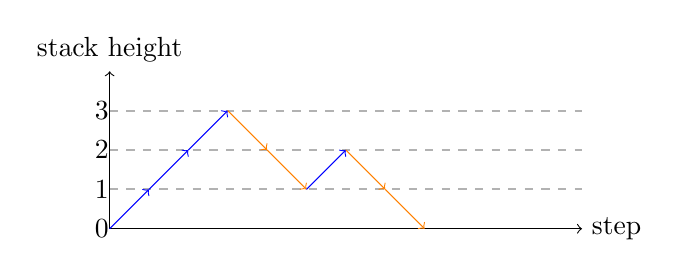
\begin{tikzpicture}
    \draw[thick, dashed, opacity=0.3] (0,0.5) -- (6,0.5);
     \draw[thick, dashed, opacity=0.3] (0,1) -- (6,1);
      \draw[thick, dashed, opacity=0.3] (0,1.5) -- (6,1.5);
      \draw[->] (0,0) -- (6,0) node[right] {step};
      \draw[->] (0,0) -- (0,2) node[above] {stack height};
     \draw[->, blue] (0,0) -- (0.5,0.5);
      \draw[->, blue] (0.5,0.5) -- (1,1);
      \draw[->, blue] (1,1) -- (1.5,1.5);
       \draw[->, orange] (1.5,1.5) -- (2,1);
    \draw[->, orange] (2,1) -- (2.5,0.5);
    \draw[->, blue] (2.5,0.5) -- (3,1);
    \draw[->, orange] (3,1) -- (3.5,0.5);
 \draw[->, orange] (3.5,0.5) -- (4,0);
\node (null) at (-0.1, 0) {0}; 
\node (one) at (-0.1, 0.5) {1}; 
\node (two) at (-0.1, 1) {2}; 
\node (three) at (-0.1, 1.5) {3}; 
    \end{tikzpicture}
\caption{Stack heights during the run of PDA.}
\label{oscb}
\end{figure}


PDA run $r$ is \textit{k-oscillating} if the harmonic of order $k$ is the greatest harmonic that is contained in $r$. \textit{Bounded-oscillation languages} are languages accepted by pushdown automata restricted to k-oscillating runs. It is important that the problem whether a given CFL is a bounded-oscillation language is undecidable \cite{BoundOsc}.
\begin{example}
Consider Figure \ref{oscb}. It shows how the stack height changes during the run of a PDA. Corresponding well-nested word is $\bar{a}\bar{a}\bar{a}aa\bar{a}aa$. The greatest harmonic in this word is order 1 harmonic (moves forming harmonic are marked in bold): $\bar{a}\bar{a}\mathbf{\bar{a}a}a\mathbf{\bar{a}a}a$, therefore oscillation of the run is 1.
\end{example}


Oscillation of the run is closely related with the $dimension$ of the corresponding parse tree. For each node $v$ in a tree $T$ a dimension $dim(v)$ is inductively defined as follows:
\begin{itemize}
\item If $v$ is a leaf, then $dim(v)$ = 0
\item If $v$ is an internal node with $k$ children $v_1, v_2, ..., v_k$ for $k \ge 1$, then 
$$
dim(v) = 
 \begin{cases}
   \max_{i \in \{1...k\}}dim(v_i) &\text{if there is a unique maximum}\\
   \max_{i \in \{1...k\}}dim(v_i)+1 &\text{otherwise}
 \end{cases}
$$
\end{itemize}


Dimension of a parse tree $T$ $dim(T)$ is a dimension of it's root.  It is observable from the definition that dimension of a tree $T$ is the height of the largest perfect binary tree, which can be obtained from $T$ by contracting edges and accordingly identifying vertices. A tree with dimension $dim(T) = 2$ is illustrated in Figure \ref{oscbtree}.


It is known that the dimension of parse trees and the oscillation defined on PDA runs are in linear relationship.

\begin{lemma}[\cite{BoundOsc}]
\label{boscdim}
Let a grammar $G = (\Sigma, N, P, S)$ be in Chomsky normal form and let $T$ be a parse tree of $G$. Then $osc(T) - 1 \le dim(T) \le 2osc(T)$.
\end{lemma}

Before we consider the value of the rational index for $k$-bounded-oscillation languages, we need to prove the following.
\begin{figure}
\begin{tikzpicture}[
level 1/.style={sibling distance=3cm},
level 2/.style={sibling distance=1.5cm}]
%\tikzstyle{every node}=[circle,draw]

\node[circle,draw] (Root) [ fill=red, red] {}
    child {
    node[circle,draw, blue] (l) {} 
    child { node[circle,draw, fill=red, red](ll) {}
            child { node[circle,draw, blue] (p) {} }
            child { node[circle,draw, blue] (pl) {} }
             }
    child { node[circle,draw, blue](lr) {} 
          child { node[circle,draw, blue] (plr) {} }
      }
}
child {
    node[circle,draw,  fill=red, red] (r) {}
    child { node[circle,draw, blue] (rl) {}} 
    child { node[circle,draw, blue] (rr) {} }
};
\node  [right=0.05cm of p] {0};
\node  [right=0.1cm of Root] {$2, dim(T)=2$};
\node  [right=0.05cm of l] {1};
\node  [right=0.05cm of r] {1};
\node  [right=0.05cm of ll] {1};
\node  [right=0.05cm of lr] {0};
\node  [right=0.05cm of pl] {0};
\node  [right=0.05cm of plr] {0};
\node  [right=0.05cm of rl] {0};
\node  [right=0.05cm of rr] {0};
\end{tikzpicture}
\caption{A tree $T$ with $dim(T)=2$. Nodes having children without unique maximum are filled.}
\label{oscbtree}            
\end{figure}
\begin{lemma}
\label{lem:treeheight}
Let  $G = (\Sigma, N, P)$ be a context-free grammar,  $D=(V, E, \Sigma)$ be a directed labelled graph with $n$ nodes. Let $w$ be the shortest string in $L(G)\cap L(D)$. Then a height of a parse tree for $w$ does not exceed $|N|n^2$.
\end{lemma}

\begin{proof}
 Assume that the parse tree for $w$ has a height of more than $|N|n^2$. There are $|N|n^2$ unique labels $(A, i, j)$ for nodes of the parse tree, so according to the pigeonhole principle, the parse tree for $w$ contains at least one subtree $T$ with label $(A, i, j)$ at the root, which has a subtree $T'$ with the same label. Then we can change $T$ with $T'$ and get a new string $w'$ which is shorter than $w$. But $w$ is the shortest, then we have a contradiction.

\end{proof}
From Lemma \ref{lem:treeheight} we have that rational index of linear languages is in $O(n^2)$. 
\begin{lemma}
\label{oscbnddim}
Let $G$ be a grammar $G = (\Sigma, N, P, S)$ in Chomsky normal form, such that every parse tree $T$ has $dim(T) \le d$, where $d$ is some constant. Let $D=(V, E, \Sigma)$ be a directed labelled graph with $n$ nodes. Then $\rho_{L(G)}$ is in $O({(|N|n^2)}^d)$.
\end{lemma}
\begin{proof}
Proof by induction on dimension $dim(T)$.
\\
\textbf{Basis.} $dim = 1$.
\\
Consider the worst-case tree $T$ with the dimension $dim(T) = 1$. The root of the tree has the same dimension and has two children (because the grammar in Chomsky normal form). There are two cases:  first, when both of child nodes have dimension equal to 0, then the tree has only two leaves and second, when one of children has a dimension 1, and the second child has a dimension equal to 0. For the second case we can recursively construct a tree of maximum height $|N|n^2$ (Lemma \ref{lem:treeheight}). Every internal node of such tree has two children, one of which has dimension equal to 0 and therefore has only one leaf. This tree is exactly the worst-case tree for linear grammar in Chomsky normal form, so the number of leaves in such tree is $O(h) = O(|N|n^2)$, where $h$ is the height of the tree. 
\\
\textbf{Inductive step.} $dim = d + 1$.
\\
Assume that $\rho_{L(G)}$ is no more than $O(h^{d})$ for every $d$, where $h$ is the height of the tree. We have two cases for the root node with dimension equal to $d+1$: 1) both of children have a dimension equal to $d$, then by proposition the tree of heght $h$ has no more than $O(h^{d})$ leaves; 2) one of children has a dimension $d + 1$, and the second child $v$ has a dimension $dim(v) \le d$. Again, a tree of maximum height with the maximum number of leaves can be constructed recursively:  each node of such tree has two children $u$ and $v$ with dimension $d+1$ and $d$ respectively (the more value of dimension of the node, the more leaves in the corresponding tree). By proposition we have no more than $(h-1)^d + (h-2)^d + (h-3)^d + ... + 1 = O(h^{d+1})$ leaves, so proposition holds for $dim = d+1$. Finally, we have $\rho_{L(G)}$ is no more than $O(h^{d}) = O({(|N|n^2)}^d)$ for every $d$.
\end{proof}
Combining Lemma \ref{boscdim} and Lemma \ref{oscbnddim}, we can deduce the following.
\begin{theorem}
\label{oscbndosc}
Let $L$ be a $k$-bounded-oscillation language with grammar $G = (\Sigma, N, P, S)$ in Chomsky normal form and $D=(V, E, \Sigma)$ be a directed labelled graph with $n$ nodes. Then $\rho_{L(G)}$ is in $O((|N|n^2)^{k/2})$.
\end{theorem}

As we can see from the proof above, the family of linear languages is included in the family of bounded-oscillation languages. The reason is that the family of bounded-oscillation languages generalizes the family of languages accepted by finite-turn pushdown automata \cite{BoundOsc}. It is interesting that for arbitrary CFL, particularly for $D_2$, the value of osciillation is not constant-bounded: it depends on the length of input and does not exeed $O(\log n)$ for the input of length $n$ \cite*{Gundermann, Wechsung}. However, for some previously studied subclasses of context-free languages,  oscillation is bounded by a constant.

\begin{example}[Superlinear languages \cite{superlinear}.]
\\
A context-free grammar $G = (\Sigma, N, P, S)$ is \textit{superlinear} if all productions of $P$ satisfy these conditions:
\begin{enumerate}
\item there is a subset $N_L \subseteq N$ such that every $A \in N_L$ has only linear productions $A\rightarrow aB$ or $A\rightarrow Ba$, where $B \in N_L$ and $a \in \Sigma$.
\item if $A \in N \setminus N_L$, then $A$ can have non-linear productions of the form $A \rightarrow BC$ where $B\in N_L$ and $C \in N$, or linear productions of the form $A\rightarrow \alpha B$ | $B \alpha$ | $\alpha$ for $B \in N_L$, $\alpha \in \Sigma^*$.
\end{enumerate}
From the grammar $G$ it is observable that its parse trees have dimension at most 2. From 
Lemma~\ref{oscbnddim}, if dimensions of all parse trees are bounded by some $k$ then the rational index of such language is polynomial, so CFL-reachability problem for superlinear languages and an arbitrary graph is in NC. 
\end{example}
\begin{figure}
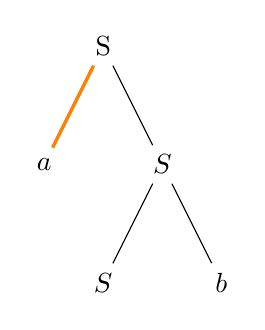
\begin{tikzpicture}
\node{S}
 child [very thick, orange] {node [black] {$a$} }
 child {node {$S$}
      child {node {$S$}}
     child {node {$b$}}
         };
\end{tikzpicture}
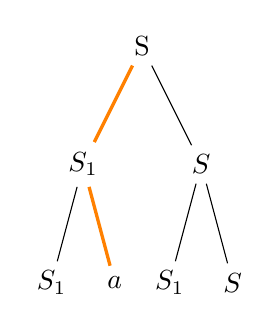
\begin{tikzpicture}[level 2/.style={sibling distance=8mm}]
\node{S} 
child [very thick, orange]  {node [black]  {$S_1$}
     child  [thin, black] {node {$S_1$}}
     child {node [black] {$a$}}
}
child  {node {$S$}
    child {node {$S_1$}}
    child {node {$S$}}
};
\end{tikzpicture}
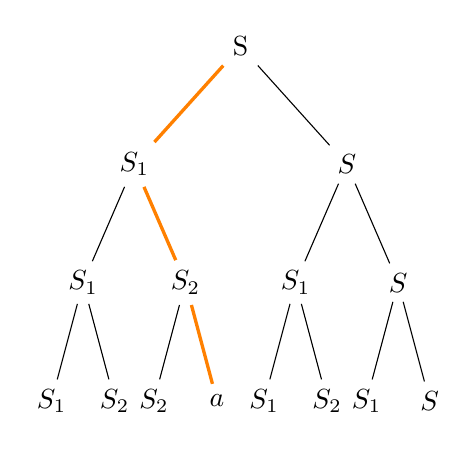
\begin{tikzpicture}[level 1/.style={sibling distance=27mm}, level 2/.style={sibling distance=13mm},  level 3/.style={sibling distance=8mm}]
\node{S} 
child [very thick, orange]  {node [black]   {$S_1$}
     child  [thin, black] {node {$S_1$} 
             child {node {$S_1$}}
             child {node {$S_2$}
                }}
     child {node [black]   {$S_2$}
                 child [thin, black] {node {$S_2$}}
                child {node [black]   {$a$}}
               }
}
child  {node {$S$}
    child {node {$S_1$}
                       child {node {$S_1$}}
             child {node {$S_2$}}
}
    child {node {$S$}
             child {node {$S_1$}}
             child {node {$S$}
                }}
};
\end{tikzpicture}
\caption{A parse trees and critical paths for piecewise linear grammars in the Chomsky normal form for $|N| = 1, 2, 3$.}
\label{crit}      
\end{figure}
\begin{example}[Piecewise linear languages.]
\\
The family of piecewise linear queries is known to be a large class of Datalog queries which have polynomial fringe property \cite{Ullman}. Those queries can be described via piecewise linear grammars. A grammar $G = (\Sigma, N, P, S)$ is \textit{piecewise linear} if every nonterminal symbol $A \in N$ generates a derivation with at most one $A$ by any sequence of applying the production rules. A piecewise linear language is a language generated by piecewise linear grammar. We show that the family of piecewise linear languages is subclass of bounded-oscillation languages by the following Lemma.
\begin{lemma}
Let  $G = (\Sigma, N, P, S)$ be a piecewise linear grammar in Chomsky normal form. Then $dim(T) \le |N| + 1$ for every parse tree $T$ of $G$.
\end{lemma}
\begin{proof} Recall that dimension of a parse tree is the maximum height of its perfect binary subtree. Let a \textit{critical path} be the longest path in parse tree, such that all nonterminals along this path are distinct. The length of the critical path is obviously bounded by the number of nonterminals of grammar.  Consider parse tree $T$ of $G$ and its arbitrary subtree $T'$. We show that every perfect binary subtree $T'$ has a critical path. Suppose that the root of $T'$ is labelled by some nonterminal $S$. The root has two children. One of the children and its descendants can not be labelled by $S$, otherwise $G$ is not piecewise linear. Thus such child should have a different label $S_1$. Consider the subtree $T''$ of $T'$ rooted by $S_1$. The root of $T''$ should have child, which is not labelled by $S$ and $S_1$, so it is labelled by a distinct nonterminal $S_2$. Going from up to down, a distict nonterminal should be used until the path ends with a terminal symbol. So, such path is critical. Examples of parse trees and critical paths in them are shown in Figure~\ref{crit}. If $T'$ is a perfect binary tree, its height is bounded by the length of the critical path. This completes the proof.
\end{proof}


\end{example}

